\chapter{Theoretische Grundlagen}


\section{Siliziumdetektoren}

Die im Silzium vorkommenden Elektronen wechselwirken mit anderen Elektronen und
Kernen des Kristalls, wodurch es zu vielen Aufspaltungen des Energieniveaus dieser kommt. Wegen dem Pauli-Prinzip können
die Elektronen nicht dieselben Quantenzahlen besitzen, wodurch sich deren Energieniveaus voneinander unterscheidet.
Die Zustände liegen dicht bei einander, weshalb von Energiebändern gesprochen wird.
Das höchste von den Elektronen besetzte Band im Grundzustand ist das Valenzband, welches von dem
nächsthöheren Band durch eine Bandlücke getrennt ist. Elektronen können
durch Anregungen in das Leitungsband wandern und somit Strom leiten, vorausgesetzt
die Anregungen sind größer als die Energielücke.

Das Einbringen von Fremdatomen in den Siliziumkristall kann dessen Eigenschaften ändern
und wird Dotierung genannt.
Hat das Fremdatom mehr oder weniger Valenzelektronen als das Silizium, ersetzt ein neuer Zustand innerhalb der Bandlücke
einen alten Zustand .
Durch Donatoren wird es für Elektronen einfacher in das Leitungsband zu wandern. Aktzeptoren
erschaffen ein Loch über dem Valenzband, welches durch ein Elektron gefüllt wird und somit ein
Loch im Valenzband zurückbleibt.
Bei den Fremdatomen wird zwischen Donatoren und Akzeptoren unterschieden, wobei die
Ersteren mehr Valenzelektronen als das Silizium besitzen und die Zweiteren weniger.
Bereiche des Siliziumkristalls mit Donatoren werden n-Dotierte Halbleiter
und Bereiche mit Akzeptoren p-Dotierte Bereiche genannt.

Bei einem Übergang von einer n-Dotierten zu einer p-Dotierten Schicht rekombinieren
die Elektronen der n-Dotierten Schicht mit den Elektronenlöchern der p-dotierten Schicht, da beide
in die anderen Bereiche diffundieren. Durch die übrig bleibenden ortsfesten Atomkerne
baut sich ein elektrisches Feld auf, welches dem Diffusionsstrom entgegenwirkt.
Ein sich einstellendes Gleichgewicht führt zu einer raumladungsträgerfreien Zone bei
dem p-n-Übergang.
Für Detektoren werden die beiden Schichten unterschiedlich stark dotiert, wobei eine
stark dotierte Oberfläche und ein leicht dotierter Bulk verwendet. Durch die asymmetrische
Dotierung breitet sich die Depletionszone hauptsächlich in den schwächer dotierten Bulk aus.
Im Falle von ($N_{\mathrm{A}} \gg N_{\mathrm{D}}$) lässt sich die Depletionstiefe $d$ beschreiben durch:
\begin{align}
  d \approx \sqrt{\frac{2 \epsilon \epsilon_0}{e} (U_{\mathrm{bi}}+U_{\mathrm{ext}})\frac{1}{N_{\mathrm{D}}}}.
\end{align}
Hierbei beschreibt $\epsilon \epsilon_0$ die Permittivität, $e$ die elementar Ladung, $N_{\mathrm{D}}$ die Donatorenkonzentration, $U_{\mathrm{bi}}$ (built-in voltage)  die
durch die festen Raumladungen entstehende Spannung und $U_{\mathrm{ext}}$ die extern angelegte Spannung. Für strahlenbeschädigte Detektoren entspricht ...


Durch eine äußere negative Spannung  an der p-Seite im Bezug zur n-Seite, oder umgekehrt, wird die Zone vergrößert und dient als Ionisationskammer für einfallende Teilchen,. Diese streuen
an den Atomkernen in der Zone und geben ein Teil oder ihre gesamte Energie bei dem Durchgang durch den Detektor ab. Mit der so abgegebenen
Energie werden Elektron-Loch Paare erzeugt, welche sich durch das vorhandene elektrische Feld zu ihrer jeweiligen dotierten
Schicht bewegen und über Elektroden als elektrisches Signal gemessen werden können.
Die raumladungsfreie Zone dient somit als Detektor und soll ein möglichst großes Volumen umfassen.

Mehr Informationen über Halbleiter finden sich in  \cite{semiconductor}.

\section{Strahlenschäden}
Wechselwirkungen von Teilchen mit Silizium können zu Defekten in deren
Gitterstruktur führen.
Die Energie der Teilchen wird dabei durch Ionisation und elastischer Streuung an den Gitteratomen abgeben. Die Ionisation der
Gitteratome wird "Total Ionizing Dose" (TID) genannt und führt zu keinen Schäden im Bulk, lediglich das Streuen der Strahlung an den
Atomkernen kann zu Defekten im Gitter führen.
Es muss zwischen verschiedenen Arten von Defekten unterschieden werden. Die Teilchen können ein Gitteratom aus dem
Gitter herausschlagen, wodurch eine Leerstelle und ein Zwischengitteratom entstehen. Das herausgeschlagene Atom
kann Silizium, aber auch ein Fremdatom sein. Daraus folgt eine Änderung der Dotierungskonzentration im
Halbleiter und somit eine Änderung seiner Eigenschaften. Somit können zum Beispiel neue Zustände innerhalb der
Bandlücke entstehen, welche Elektronen und Löcher einfangen  und emitieren, wodurch der Leckstrom wächst.
Zwischengitteratome können stabile Komplexe mit einander bilden. Diese werden nicht durch Annealing
beeinflusst und verändern die Halbleiter permanent.

Die durch Strahlenschäden hervorgerufenen Energiezustände verhalten sich hauptsächlich wie Akzeptoren im Siliziumgitter. Bei
einer steigenden Anzahl an Defekten werden die dotierten Schichten insgesamt positiver. Für die n-dotierte Schicht kann
es zur sogennaten Typinversion kommen, wodurch diese sich in eine leicht p-dotierte Schicht umwandelt. Bei einer
solchen Typinversion wird die Dotierungskonzentration minimal und die benötigte externe Spannung für das Depletieren des Sensors geht gegen Null, da sich
das Vorzeichen der Ladung der Verarmungszone ändert.
Für größer werdende Fluenzen steigt die benötigte externe Spannung und die
Dotierungskonzentration kontinuierlich an.
In Abbildung \ref{fig:typeinversion} ist eine Typinversion aus dem Buch "Teilchendetektoren" dargestellt.

\begin{figure}
    \includegraphics[width=0.83\textwidth]{build/typeinversion.PNG}
\caption{Depletionsspannung und Dotierungskonzetration in Abhängigkeit von der Fluenz \cite{semiconductor}.}
\label{fig:typeinversion}
\end{figure}

Nach der "Non-Ionizing Energy Loss" (NIEL) Hypothese wird der Detektorschaden durch die Energie des herausgeschlagenen
Atoms beschrieben und ist unabhängig von der ursprünglichen Wechselwirkung.
Um somit Fluenzen $ \Phi$ von verschiedenen Teilchen (Lepton, Hadron) miteinander vergleichen zu können, werden diese
auf eine $\SI{1}{\mega\eV}$ Neutronstrahlung normalisiert und haben die Einheit $[\Phi_{\mathrm{eq}}]\mathrm{\frac{n_{\mathrm{eq}}}{cm^2}}$.


\section{Annealing der Dotierungskonzentration}
Annealing beschreibt im Allgemeinen die durch Erhitzung hervorgerufenen Veränderungen von Materialeigenschaften. Für strahlengeschädigte
Halbleiter werden dabei, durch die zugeführte Wärme, die Defekte teilweise behoben werden, um somit eine
bessere Funktionsfähigkeit über einen längeren Zeitraum zu garantieren. Die auftretenden Effekte sind dabei wie folgt:

\textbf{1. Migration:} Ist die Temperatur hoch genug können die Zwischengitteratome durch das Gitter wandern und
Leerstellen im Gitter füllen.

\textbf{2. Komplexformation:} Das Migrieren der Atome kann zum Ausbilden von Komplexen führen. Dies geschieht durch das
Gruppieren von mehreren Zwischengitteratomen im Kristall.

\textbf{3. Dissoziation:} Komplexe können bei hohen Temperaturen Dissoziieren, wodurch einzelne Bestandteile des Komplexes
durch das Gitter migrieren können. Dafür muss die Schwingungsenergie des Gitters größer als die Bindungsenergie der Komplexe sein.

Die Annealingeffekte bewirken eine Änderung in der effektiven Dotierungskonzentration
\begin{align}
  N_{\mathrm{eff}}= |N_{\mathrm{D}}-N_{\mathrm{A}}|,
\end{align}
welches durch das Hamburger Modell beschrieben wird.
Die Änderung von $N_{\mathrm{eff}}$ ist gegeben durch:
\begin{align}
  \Delta N_{\mathrm{eff}}(t, \Phi_{\mathrm{eq}}, T)   = N_{\mathrm{C}}(\Phi_{\mathrm{eq}}) + N_{\mathrm{A}}(t, \Phi_{\mathrm{eq}}, T) + N_{\mathrm{Y}}(t, \Phi_{\mathrm{eq}}, T) \text{\cite{moll}}
  \label{eqn:N_eff}
\end{align}
Die einzelnen Summanden werden im folgenden erläutert.

\textbf{\textit{Stable Damage}} $\symbf{N_{\mathrm{C}}}:$ Der stable Damage ist unabhängig von der Temperatur und wird durch Annealing nicht beeinflusst.
\begin{align}
  N_{\mathrm{C}}(\Phi_{\mathrm{eq}}) = N_{\mathrm{C0}}[1-\exp{(-c \cdot \Phi_{\mathrm{eq}})}] + g_{\mathrm{c}} \cdot \Phi_{\mathrm{eq}}
\end{align}
Der erste Summand folgt aus einer unvollständigen Entfernung von Donatoren, der zweite Summand beschreibt stabile Defekte, welche sich wie Akzeptoren verhalten \cite{beyer}.
Hierbei beschreibt $N_{\mathrm{C0}}$ die Amplitude, $g_{\mathrm{c}}$ die sogenannte "introduction rate" der Akzeptoren und $c$ einen Fitparameter.

\textbf{\textit{Shortterm annealing}} $\symbf{N_{\mathrm{A}}}:$ Das shortterm annealing bewirkt eine Verringerung der Dotierungskonzentration und entsteht durch
das Annealing von Akzeptoren, was zu einer kleineren Dotierungskonzentration führt. . Dieser Effekt wird beim
gezielten Ausheilen des Sensors ausgenutzt. Die Bezeichnung rührt daher, dass $N_{\mathrm{A}}$ meistens in den ersten 100 Minuten verschwindend gering wird. Die
Funktion wird näherungsweise beschrieben durch:
\begin{align}
  N_{\mathrm{A}}(t, \Phi_{\mathrm{eq}}, T) = \Phi_{\mathrm{eq}} \cdot g_{\mathrm{a}} \cdot \exp{\left(-\frac{t}{\tau_{\mathrm{a}}(T)}\right)}.
\end{align}
Hierbei gilt für die temperaturabhängigen Funktion:
\begin{align}
  \tau_{\mathrm{a}}(T) = \frac{1}{k_{0\mathrm{a}}}\exp{\left(\frac{E_{aa}}{k_{\mathrm{b}}T}\right)}.
\end{align}
Mit der "introduction rate" $g_{\mathrm{a}}$, dem Frequenzfaktor $k_{0\mathrm{a}}$, der Boltzmann Konstante $k_{\mathrm{b}}$ und
der Aktivierungsenergie $E_{aa}$


\textbf{\textit{Longterm annealing}} $\symbf{N_{\mathrm{Y}}}:$ Der Aufbau von
Akzeptoren sorgen nach einem hinreichend großen Zeitraum für eine steigende
Dotierungskonzentration. Dieser Effekt wird wie folgt berechnet.
\begin{align}
  N_{\mathrm{Y}}(t, \Phi_{\mathrm{eq}}, T)     = N_{\mathrm{Y , \inf}}\cdot \left(1 - \frac{1}{1 + \frac{t}{\tau_{\mathrm{Y}}(T)}}\right)
\end{align}
Beginnend bei null läuft die Funktion asymptotisch gegen die Konstante $N_{\mathrm{Y, \inf}}$.
Für $\tau_{\mathrm{Y}}(T)$ gilt:
\begin{align}
  \tau_{\mathrm{Y}}(T) = \frac{1}{k_{0\mathrm{Y}}}\exp{\left(\frac{E_{Y}}{k_{\mathrm{b}}T}\right)}.
\end{align}
Auch hier ist $k_{0\mathrm{Y}}$ ein Frequenzfaktor und $E_{\mathrm{Y}}$ die Aktivierungsenergie. Der Faktor $N_{\mathrm{Y , \inf}}$
ist das Produkt der "introduction rate" $g_{\mathrm{Y}}$ und der Fluenz. Nach einem unendlich großen Zeitraum strebt
die Funktion $N_{\mathrm{A}}(t, \Phi_{\mathrm{eq}}, T) + N_{\mathrm{Y}}(t, \Phi_{\mathrm{eq}}, T)$ gegen $N_{\mathrm{Y , \inf}}$.
In Abbildung \ref{fig:n_eff_beispiel} ist beispielhaft das Annealingverhalten eines
Sensors dargestellt.

\begin{figure}
  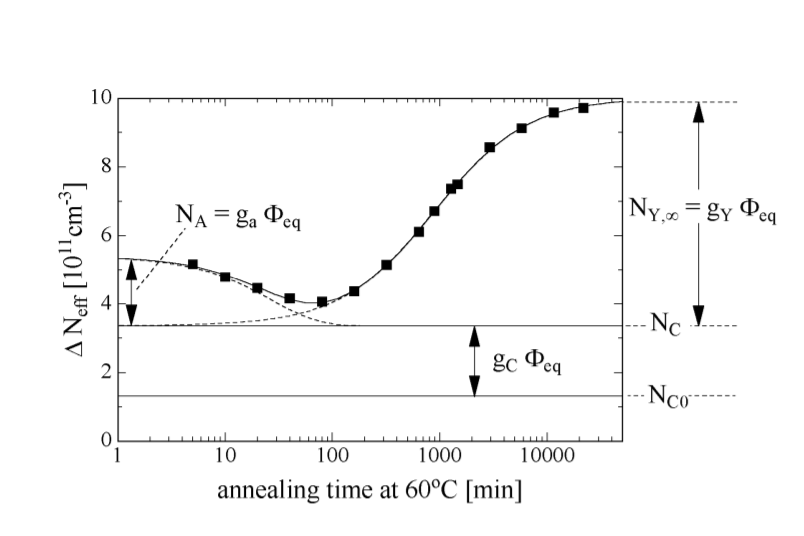
\includegraphics[width=0.83\textwidth]{logos/n_eff_beispiel.PNG}
  \caption{Dotierungskonzentration bei 60°C für eine Bestrahlung mit einer Fluenz
  von $\Phi=\SI{1.4e13}{\per\centi\meter\squared}$ .\cite{moll}}
  \label{fig:n_eff_beispiel}
\end{figure}



\section{Annealing des Leckstroms}
Der Leckstrom beschreibt allgemein einen messbaren Stromfluss über einen als isolierend
angenommenen Weg. Bei den hier thematisierten Sensoren ist damit der Strom gemeint, der trotz sperrender
Diode fließt. Dieser entsteht hauptsächlich durch die Generation von Ladungsträgern an Defekten, welche
bei realen Dioden auch vor der Bestrahlung vorhanden sind. \cite{moll}.
Durch das Annealing werden die Defekte in der Mitte der Energielücke teilweise behoben,
was zu einer Verringerung des Leckstroms führt.

Der Leckstrom vor und nach der Bestrahlung ist temperaturabhängig und wird
beschrieben durch
\begin{align}
  I(T) \propto T^2 \exp{\frac{-E_{\mathrm{g}}}{2 k_{\mathrm{B}}T}} \text{\cite{moll}} \label{eqn:Chilingarov_2013}.
\end{align}
Hier ist $E_{\mathrm{g}}$ die Energie der Bandlücke.

Die Fluenz und der durch Strahlung hervor gerufene Leckstrom $\Delta I$ sind
proportional zueinander.


\begin{align}
  \Delta I = \alpha \Phi_{\mathrm{eq}} \cdot V
\end{align}
Hierbei ist $V$ das Volumen des Detektormaterials und $\alpha$ die
sogenannte Schadensrate.



Die Verringerung des Leckstromes durch annealing wird mit der Schadensrate
beschrieben, welche als eine Funktion abhängig von der Zeit und
Temperatur beschrieben wird.\cite{moll}

\begin{align}
  \alpha(t, T) = \underbrace{\alpha_I \cdot \exp{\left(-\frac{t}{\tau_{\mathrm{I}}(T)}\right)}}_{\mathrm{shortterm \: annealing}} + \underbrace{\alpha_{\mathrm{0}}(T) -\beta \cdot \ln{\left(\frac{t}{t_{\mathrm{0}}}\right)}}_{\mathrm{longterm \: annealing}} \text{\label{eqn:damage}}
\end{align}
Mit den Fitparameter $\alpha_I$,  $\beta$, den in \cite{moll} berechnete Werten für den Fitparameter $\alpha_{\mathrm{0}}(T)$, sowie der
temperaturabhängigen Funktion $\tau_{\mathrm{I}}(T)$:
\begin{align}
  &\alpha_{\mathrm{0}}(T) = \SI{-8.9e-17}{\ampere\per\centi\meter} + \SI{4.6e-14}{\ampere\kelvin\per\centi\meter} \cdot \frac{1}{T} \\
  &\tau_{\mathrm{a}}(T) = \frac{1}{k_{0\mathrm{I}}}\exp{\left(\frac{E_{I}}{k_{\mathrm{b}}T}\right)}
\end{align}
Wie für $N_{\mathrm{A}}$ und $N_{\mathrm{Y}}$ ist $k_{0\mathrm{I}}$ ein Frequenzfakor und $E_{I}$ die Aktvierungsenergie.

Anders als das Annealingverhalten der Dotierungskonzentration kann die Schadensrate
bei fortschreitendem annealing nur sinken. Für kurze und
lange Zeiten dominieren in diesem Modell wie bei der Dotierungskonzentration unterschiedliche
Terme. Für große Temperaturen und Zeiten würde die Schadensrate kleiner als null
werden. Die Messwerte für kleine $\alpha$ weichen jedoch von den
Vorhersagen des Modells ab und nähern sich einen Wert größer null an. Auch für große Schadenraten ab ungefähr $\alpha=\SI{6e-17}{\ampere\per\centi\meter}$
versagt das Modell.
Dies ist in Abbildung \ref{fig:damage_rates} dargestellt.

\begin{figure}
  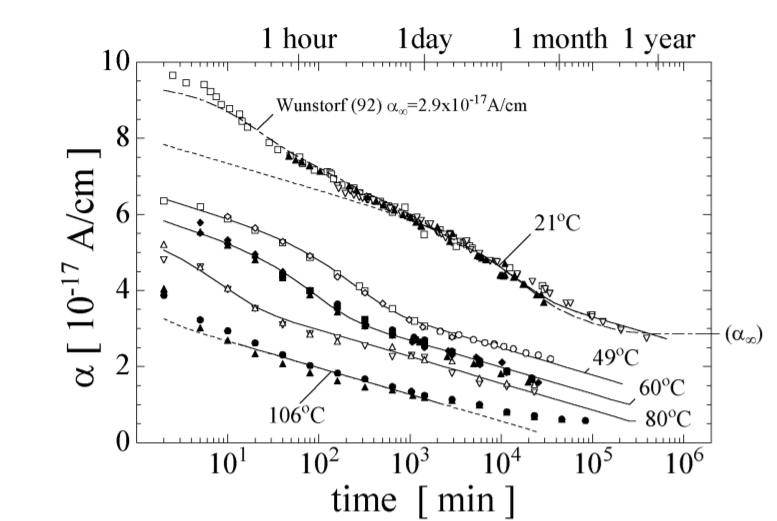
\includegraphics[width=0.83\textwidth]{logos/schadensraten.PNG}
  \caption{Schadensraten für verschiedene konstante Annealingtemperaturen.\cite{moll}}
  \label{fig:damage_rates}
\end{figure}
